\section{Construction of $\psi$}
\label{sec:psi}

This section closely follows \cite[Appendix A]{calegari2024linear}.
To get a contradiction, we need to choose $\varphi: (\overline{\bD},0) \to (\bC, 0)$ which makes the holonomy bound smaller than 14.
We will assume that $\varphi$ is of the form $\varphi = h \circ \psi$ where $\psi: \bD \to \Omega \subset \bD$ and $h$ is the hauptmodul of $Y_0(2)$ given by
\begin{equation}
\label{eqn:h}
     h := \lambda + \frac{\lambda}{\lambda - 1} = -256 q \prod_{n=1}^{\infty} (1 + q^n)^{24} = -256 \frac{\Delta(2\tau)}{\Delta(\tau)}, \quad q = e^{2\pi i \tau}.
\end{equation}
Then we need to choose $\varphi$ so that
\begin{enumerate}
    \item the image of $\psi$ inside $\bD$ avoids all the preimages of $-\frac{1}{72}$ under $h$ except for the one preimage $0.0000541\dots \in \bR$ (unique preimage in $\bR$),
    \item the bound from Theorem \ref{thm:bound} is smaller than 14.
\end{enumerate}
In other words, we want $\Omega$ to have sufficiently large conformal radius which make $|\psi'(0)|$ as large as possible.
Also, we want to make $\psi$ small enough so that the integral on the numerator is not too large.
The condition 1 is required to ensure holomorphicity of the pullbacks of our 14 functions via Proposition \ref{prop:pullbackhol} (more precisely, we can get a univalence from it).
To obtain this, we construct $\psi$ as a composition of two basic type of conformal maps: \emph{lunes} and \emph{slits}\footnote{In \cite{calegari2024linear}, \emph{gobbles} (composition of two lunes) are also introduced, but we will not use it.}.

\emph{Lune} is a conformal map that removes a part of a disk from a larger disk.
For $c > 1$, the map
$$
    f(z, c) = z \cdot \frac{(c^2 + 1) + (c^2 - 1)z}{(c^2 - 1) + (c^2 + 1)z}
$$
maps a Lune
$$
    L(c) := \bD \backslash \left(\bD \cap D \left(-\frac{c^2 + 1}{c^2 - 1}, \frac{2c}{c^2 - 1}\right)\right)
$$
to the unit disk $\bD$ biholomorphically (note that boundaries of two disks intersect at right angles).
It has an explicit inverse map $h(z, c): \bD \to L(c)$ that maps $\bD$ to a lune \cite[Equation A.1.1]{calegari2024linear}, and the conformal radius of $L(c)$ is $\frac{c^2 - 1}{c^2 + 1}$.

\emph{Slit} is a conformal map that removes a line segment from a disk.
For a real number $0 < r < 1$, we have an explicit conformal map \cite[Equation A.3.1]{calegari2024linear}
$$
    \Slit(z, r) : (\bD, 0) \xrightarrow{\simeq} (\bD \backslash (-1, r], 0),
$$
and one can check that $\bD \backslash (-1, r]$ has a conformal radius $|\Slit'(0, r)| = \frac{4r}{1 + r^2}$.

Now, we construct $\varphi$ (hence $\psi$) via lunes and slits as follows.
I'll write a formula first:
\begin{equation}
\label{eqn:psi}
    \psi(z) = -R \cdot h(-e^{2\pi i \theta_1} \cdot \Slit (e^{2\pi i \theta_2} \cdot \Slit(e^{2 \pi i \theta_3} \cdot \Slit (e^{2\pi i \theta_4} \cdot \Slit (c' z, r_1), r_2), r_3), r_4), c)
\end{equation}
where $R, c, c', \theta_i, r_i$ are some parameters to be determined later.
We first choose $R = 0.77$ so that we can avoid all the unwanted preimages except for the 4 points which are not real and closest to the origin (we can check this value rigorously by passing back to $\bH$ and consider $\Gamma_0(2)$ orbits).
The lune map (with $c = 7.5$) is used to remove a (right) part of $\bD$ where $h(z)$ takes large values.
At last, the remaining 4 preimages are removed via slit maps and rotations, one by one.
$c' = 0.995$ is chosen to make sure that the preimages are excluded.
Note that we don't have easily expressible maps which does all the procedure above at once, and that's why we use composition of lune and slit maps (which also explains asymmetry of the resulting contour $\psi(\bT)$\footnote{Comment from the talk: if you compose more than one slit maps, then the corresponding slits will be curved a bit.}).
Since all the maps and the parameters above are explicit, we can compute the exact value of the conformal radius.


\begin{figure}[htp] 
\label{fig:psi}
    \centering
    \subfloat{%
        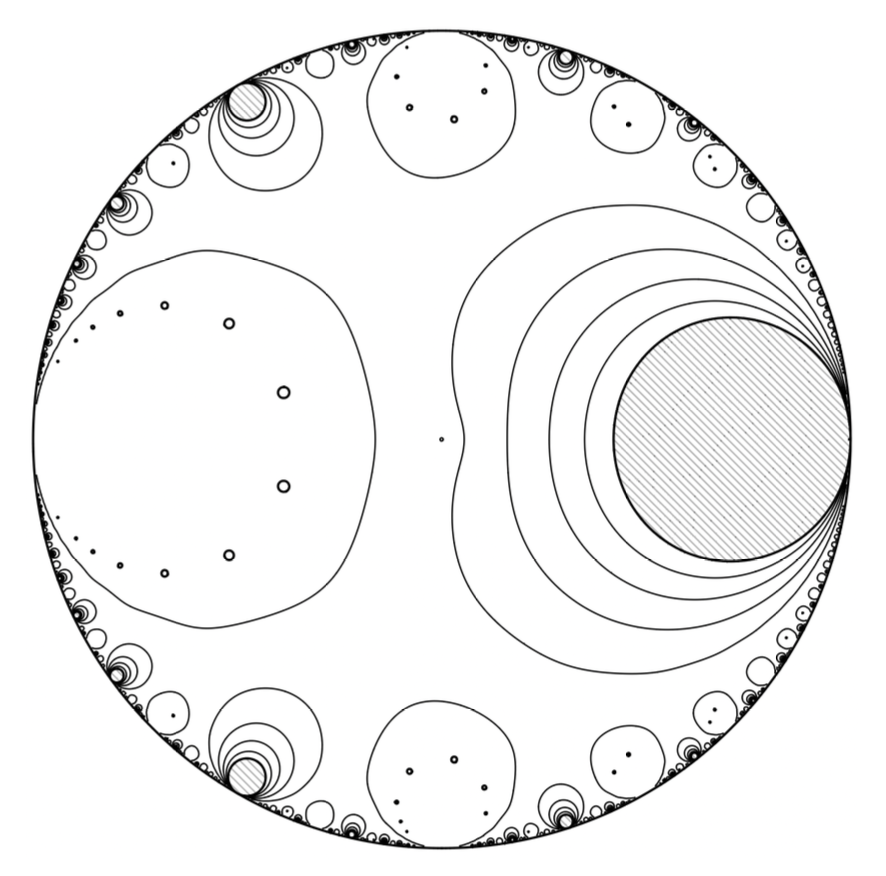
\includegraphics[width=0.45\textwidth]{src/psi1.png}%
        \label{fig:a}%
        }%
    \hfill%
    \subfloat{%
        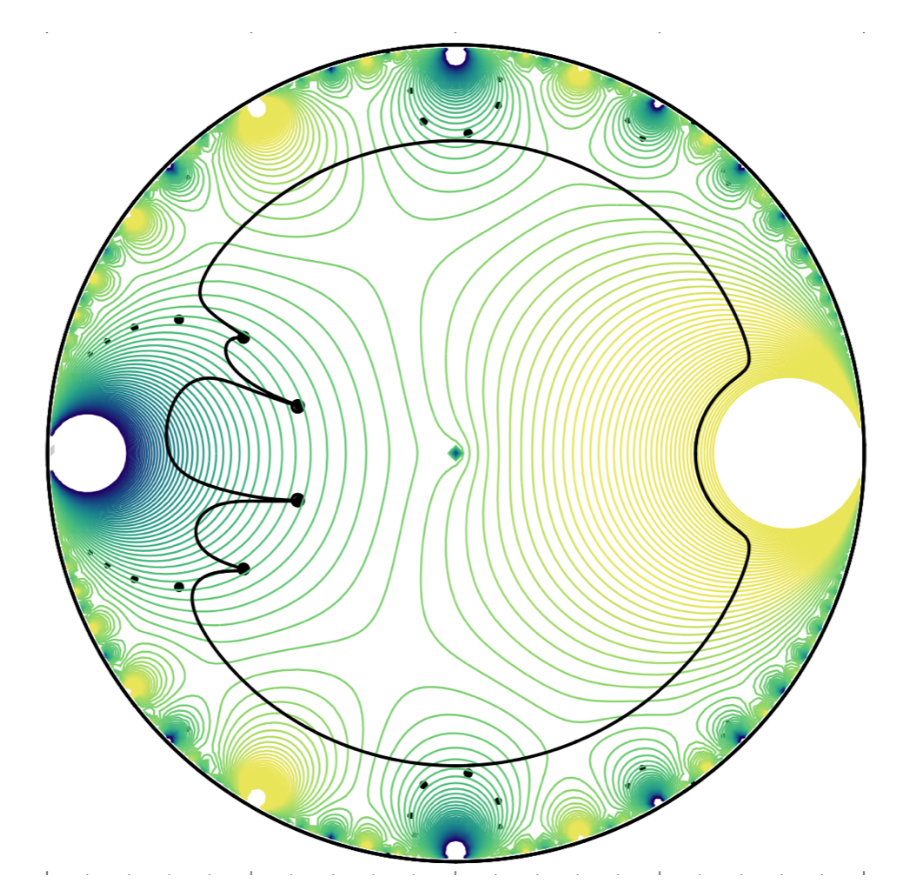
\includegraphics[width=0.47\textwidth]{src/psi2.png}%
        \label{fig:b}%
        }%
    \caption{Topography of $h$ (left, \cite[A.0.3]{calegari2024linear}) and the contour $\psi(\bT)$ (right, \cite[Figure A.4.5]{calegari2024linear})}
\end{figure}

\newpage